\documentclass[12pt]{report}
\usepackage[utf8]{inputenc}
\usepackage[top=2cm, bottom=2cm, left=2cm, right=2cm]{geometry}
\usepackage[francais]{babel}
\usepackage[T1]{fontenc}
\usepackage{graphicx}
\usepackage{subcaption}

% charte graphique non respectée pour le moment

\title{Développement d'une bibliothèque mathématique performante pour le traitement d'images médicales}
\author{Elève ingénieur : François PIAT}
\date{Année scolaire 2015-2016}

\begin{document}
	
\maketitle
\section*{Abstract/ résumé et mots-clés, Sommaire, Introduction} % dans cet ordre

\chapter{Environnement de travail} 
	\section{Le laboratoire}
	\subsection{Imperial College London - Department of computing}
	Domaine d'activité, stats, organigramme
	\subsection{BioMedIA}
	synopsis
	détail des activités du laboratoire
	
%	La mission du groupe BioMedIA est de développer de nouvelles techniques de
%	calcul pour l'analyse d'images biomédicales. Le groupe se concentre sur des
%	domaines de recherche de pointe, y compris:
%
%	- Le développement d'algorithmes d'acquisition, d'analyse et d'interprétation
%	des images. En particulier dans les domaines du recalage, de la reconstruction,
%	du suivi de mouvement, de la segmentation et de la modélisation.
%
%	- L'apprentissage machine pour l'extraction d'information clinique à partir
%	d'images médicales. Les applications incluent le diagnostic assisté par
%	ordinateur, la planification automatisée de traitement médicale, ou encore les
%	interventions et la thérapie guidées par ordinateur.
%
%	Nous nous intéressons particulièrement à l'imagerie et les technologies de
%	traitement informatique qui nous permettent de mieux comprendre le
%	développement du cerveau humain, l’évolution des maladies mentales et le
%	diagnostic des patients atteints de maladie cardiovasculaire.

	\section{Cadre du projet} présentation d'MIRTK +application +architecture(modules...)
%	 - logiciel de traitement d'image médicales, utilisé par les chercheurs en milieu médical.
%	 - stable mais nécessite une maintenance et une amélioration continue pour rester pertinent.
%	 Intervention sur le module "Numerics", bibliothèque mathématique.
\chapter{Objectifs et cahiers des charges}
	\section{Problématique} inclure contexte du projet (back-end math) dépendances externes : eigen et boost + noyaux internes implémentés via TBB => inconsistence => parrallélisation existante floue , efficacité = ? performances=? => profilage
	===> n'utiliser qu'une seule dépendance (externe) : ArrayFire qui peut amener l'optimisation via GPU (3 points majeurs)
	 

	\section{Cahier des charges}
	Arrayfire a été choisi pour palier les 3 points de la problematique
	- Intégrer ArrayFire à MIRTK, aussi bien au niveau des manipulations mathématiques qu'à celui de la programmation parallèle.
	\newline- Enlever toute dépendance de MIRTK à TBB
	\newline- (Le délivrable sera composé IDEALEMENT de 2 backends, l'un AF et l'autre EIGEN. En fonction des applications, un switch automatique entre chaque structure sera appelé en dur grâce à des commandes pré-proc.) => étape bonus
	\newline- La programmation sera réalisée de manière transparente, c'est-à-dire que MIRTK doit réaliser les mêmes fonctions et garder la même API même si le code plus en profondeur est modifié.
	\newline- Plusieurs benchmarks affirmeront les performances d'ArrayFire et de l'optimisation globale de MIRTK. (test CPU et GPU)
	
	\section{Objectifs et milestones}
	\subsection{Objectifs}- Ajouter ArrayFire à MIRTK, en remplaçant les fonctions d'EIGEN les moins adaptées par les fonctions d'AF. \newline
	- Faire un profiling des fonctions concernées par TBB, et interpréter les résultats afin d'élaborer une stratégie pour implanter la programmation // d'AF.\newline
	- Supprimer er les TBB inutiles ou peu efficaces, et remplacer les autres par l'équivalent d'AF (gfor).\newline
	
	
	\subsection{Diagramme de GANTT}
	 => gantt chart prévisionnel (à mettre en français)
	\begin{figure}[h!]
		\begin{center}
			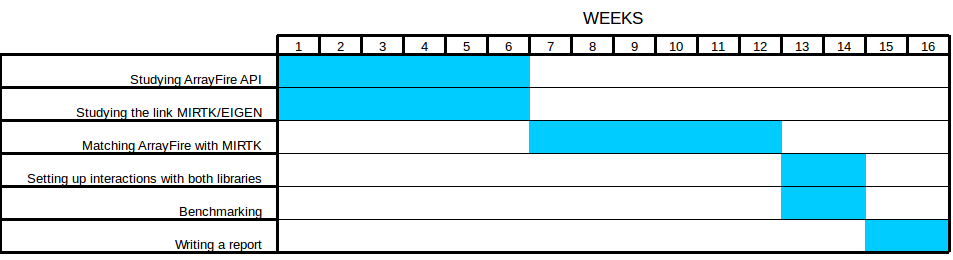
\includegraphics[width=18cm]{Reports/figures/estimated_gantt.png}
		\end{center}	
		\caption{Diagramme de GANTT prévisionnel}
		\label{Diagramme de GANTT prévisionnel}
	\end{figure}
\chapter{Réalisation}
	\section{Profilage}
	définition du profilage (merci wikipédia) + dire pourquoi c est important ici
	
	Profilage=> on identifie les fonctions sur lesquelles agir en premier
	On utilise Valgrind, qui, avec callgrind analyse la manière dont les caches sont utilisés.
	pk valgrind ?
% => projet open-source multi-plateforme et disponible dans les packages linux, autres alternatives étudiées (VTUNE intel, installation compliquée, et codeXL, qui nécessite des proc AMD).
%	
%	\newline\newline
%	Les tests ont été effectués sur une machine dont les caractéristiques sont les suivantes : \newline
%	{$\bullet$} \textit{Nombre de coeurs:} 8, 2 threads chacun\newline
%	{$\bullet$} \textit{Cadence:} 1.6 GHz \newline
%	{$\bullet$} \textit{Nombre de caches:} 4 \newline
%	{$\bullet$} \textit{Taille des caches:}32k, 32k, 256K, 8192K \newline
%	ajouter le maximum de détails (RAM, nom du proc ...)\newline
%	Pour une quantité réduite de tests, et afin de cibler les modèles d'utilisation de TBB à remplacer, on a pris l'une des fonctions les plus sollicitées dans MIRTK, il s'agit d'une fonction nommée \textit{transform-image}, et qui dispose de 5 options, définissant un type d'interpolation mathématique : Linéaire (par défaut), méthode voisin le plus proche (NN), gaussienne, sinus cardinal et B-Spline. 
	
	\subsection{Analyse du nombre d'instructions}
	
	(Placer ici des graphiques de performances)
	\subsection{Analyse des fuites de cache}
	
	(Placer ici des graphiques de performances)
	
	\section{Integration d'ArrayFire dans MIRTK}
	\subsection{Implémentation du module mathématique}
	Programmation transparente entre Eigen et ArrayFire.
	\subsection{Gestion de la programmation parallèle}
	Optimisation des threads et suppression de TBB au profit de ArrayFire.
	\newline
	Le contenus des sous-parties, ainsi que d'éventuelles d'autres sous-parties dépendront du résultat du profilage.
%	\subsection{Switch automatique de back-end}
%	Commandes prépocesseur pour indiquer au logiciel quel est le back-end à utiliser (ArrayFire ou Eigen) en fonction de l'opération souhaitée.
	\section{Benchmarking}
	- Analyse des performances obtenues \newline
	- Comparaison avec le profilage initial ? \newline
	- Points où il y a eu des concessions (exemple: alourdir le code pour parvenir à un résultat précis)
\section*{Conclusion, Sources, Table des illustrations, Glossaire, Annexes} % dans cet ordre
	
\end{document}
